%%%%%%%%%%%%%%%%%%%%%%%%%%%%%%%%%%%%%%%%%%%%%%%%%%%%%%%%%%%%%%%%%%%%%%
%%  Copyright by Wenliang Du.                                       %%
%%  This work is licensed under the Creative Commons                %%
%%  Attribution-NonCommercial-ShareAlike 4.0 International License. %%
%%  To view a copy of this license, visit                           %%
%%  http://creativecommons.org/licenses/by-nc-sa/4.0/.              %%
%%%%%%%%%%%%%%%%%%%%%%%%%%%%%%%%%%%%%%%%%%%%%%%%%%%%%%%%%%%%%%%%%%%%%%

\newcommand{\commonfolder}{../../common-files}


\documentclass[11pt]{article}

\usepackage[most]{tcolorbox}
\usepackage{times}
\usepackage{epsf}
\usepackage{epsfig}
\usepackage{amsmath, alltt, amssymb, xspace}
\usepackage{wrapfig}
\usepackage{fancyhdr}
\usepackage{url}
\usepackage{verbatim}
\usepackage{fancyvrb}
\usepackage{adjustbox}
\usepackage{listings}
\usepackage{color}
\usepackage{subfigure}
\usepackage{cite}
\usepackage{sidecap}
\usepackage{pifont}
\usepackage{mdframed}
\usepackage{textcomp}
\usepackage{enumitem}
\usepackage{hyperref}


% Horizontal alignment
\topmargin      -0.50in  % distance to headers
\oddsidemargin  0.0in
\evensidemargin 0.0in
\textwidth      6.5in
\textheight     8.9in 

\newcommand{\todo}[1]{
\vspace{0.1in}
\fbox{\parbox{6in}{TODO: #1}}
\vspace{0.1in}
}


\newcommand{\unix}{{\tt Unix}\xspace}
\newcommand{\linux}{{\tt Linux}\xspace}
\newcommand{\minix}{{\tt Minix}\xspace}
\newcommand{\ubuntu}{{\tt Ubuntu}\xspace}
\newcommand{\setuid}{{\tt Set-UID}\xspace}
\newcommand{\openssl} {\texttt{openssl}}

% Arrows
\newcommand{\pointleft}[1]{\reflectbox{\ding{217}} \textbf{\texttt{#1}}}
\newcommand{\pointright}[1]{\ding{217} \textbf{\texttt{#1}}}
\newcommand{\pointupleft}[1]{\reflectbox{\ding{218}} \textbf{\texttt{#1}}}

% Line numbers
\newcommand{\lineone}{\ding{192}\xspace}
\newcommand{\linetwo}{\ding{193}\xspace}
\newcommand{\linethree}{\ding{194}\xspace}
\newcommand{\linefour}{\ding{195}\xspace}
\newcommand{\linefive}{\ding{196}\xspace}
\newcommand{\linesix}{\ding{197}\xspace}
\newcommand{\lineseven}{\ding{198}\xspace}
\newcommand{\lineeight}{\ding{199}\xspace}
\newcommand{\linenine}{\ding{200}\xspace}


% Fancy headers
\pagestyle{fancy}
\lhead{\bfseries SEED Labs}
\chead{}
\rhead{\small \thepage}
\lfoot{}
\cfoot{}
\rfoot{}


\definecolor{dkgreen}{rgb}{0,0.6,0}
\definecolor{gray}{rgb}{0.5,0.5,0.5}
\definecolor{mauve}{rgb}{0.58,0,0.82}
\definecolor{lightgray}{gray}{0.90}


\lstset{%
  frame=none,
  language=,
  backgroundcolor=\color{lightgray},
  aboveskip=3mm,
  belowskip=3mm,
  showstringspaces=false,
%  columns=flexible,
  basicstyle={\small\ttfamily},
  numbers=none,
  numberstyle=\tiny\color{gray},
  keywordstyle=\color{blue},
  commentstyle=\color{dkgreen},
  stringstyle=\color{mauve},
  breaklines=true,
  breakatwhitespace=true,
  tabsize=3,
  columns=fullflexible,
  keepspaces=true,
  escapeinside={(*@}{@*)}
}

\newcommand{\newnote}[1]{
\vspace{0.1in}
\noindent
\fbox{\parbox{1.0\textwidth}{\textbf{Note:} #1}}
%\vspace{0.1in}
}


%% Submission
\newcommand{\seedsubmission}{You need to submit a detailed lab report, with screenshots,
to describe what you have done and what you have observed.
You also need to provide explanation
to the observations that are interesting or surprising.
Please also list the important code snippets followed by
explanation. Simply attaching code without any explanation will not
receive credits.}

%% Book
\newcommand{\seedbook}{\textit{Computer \& Internet Security: A Hands-on Approach}, 2nd
Edition, by Wenliang Du. See details at \url{https://www.handsonsecurity.net}.\xspace}

\newcommand{\seedisbook}{\textit{Internet Security: A Hands-on Approach}, 3rd
Edition, by Wenliang Du. See details at \url{https://www.handsonsecurity.net}.\xspace}

\newcommand{\seedcsbook}{\textit{Computer Security: A Hands-on Approach}, 3rd
Edition, by Wenliang Du. See details at \url{https://www.handsonsecurity.net}.\xspace}

\newcommand{\seedcibook}{\textit{Computer \& Internet Security: A Hands-on Approach}, 3rd
Edition, by Wenliang Du. See details at \url{https://www.handsonsecurity.net}.\xspace}

%% Videos
\newcommand{\seedisvideo}{\textit{Internet Security: A Hands-on Approach},
by Wenliang Du. See details at \url{https://www.handsonsecurity.net/video.html}.\xspace}

\newcommand{\seedcsvideo}{\textit{Computer Security: A Hands-on Approach},
by Wenliang Du. See details at \url{https://www.handsonsecurity.net/video.html}.\xspace}

%% Lab Environment
\newcommand{\seedenvironment}{This lab has been tested on our pre-built
Ubuntu 16.04 VM, which can be downloaded from the SEED website.\xspace}

\newcommand{\seedenvironmentA}{This lab has been tested on our pre-built
Ubuntu 16.04 VM, which can be downloaded from the SEED website.\xspace}

\newcommand{\seedenvironmentB}{This lab has been tested on our pre-built
Ubuntu 20.04 VM, which can be downloaded from the SEED website.\xspace}

\newcommand{\seedenvironmentC}{This lab has been tested on the SEED
Ubuntu 20.04 VM. You can download a pre-built image from the SEED website, 
and run the SEED VM on your own computer. However,
most of the SEED labs can be conducted on the cloud, and 
you can follow our instruction to create a SEED VM on the cloud.\xspace}

\newcommand{\seedenvironmentAB}{This lab has been tested on our pre-built
Ubuntu 16.04 and 20.04 VMs, which can be downloaded from the SEED website.\xspace}

\newcommand{\nodependency}{Since we use containers to set up the lab environment, 
this lab does not depend much on the SEED VM. You can do this lab
using other VMs, physical machines, or VMs on the cloud.\xspace}

\newcommand{\adddns}{You do need to add the required IP address mapping to
the \texttt{/etc/hosts} file.\xspace}






\newcommand{\seedlabcopyright}[1]{
\vspace{0.1in}
\fbox{\parbox{6in}{\small Copyright \copyright\ {#1}\ \ by Wenliang Du.\\
      This work is licensed under a Creative Commons
      Attribution-NonCommercial-ShareAlike 4.0 International License.
      If you remix, transform, or build upon the material, 
      this copyright notice must be left intact, or reproduced in a way that is reasonable to
      the medium in which the work is being re-published.}}
\vspace{0.1in}
}




\hypersetup{%
    pdfborder = {0 0 0}
}

\lhead{\bfseries SEED Labs -- BGP Exploration and Attack}
\newcommand{\bgpFigs}{./Figs}

% Chapter numbers in the tutorial
\newcommand{\bgpintro}{1\xspace}
\newcommand{\bgpprotocol}{3\xspace}
\newcommand{\bgppeering}{6\xspace}
\newcommand{\bgpupdate}{7\xspace}
\newcommand{\pathselection}{8\xspace}
\newcommand{\bigcommunity}{9\xspace}
\newcommand{\transitas}{10\xspace}
\newcommand{\ipanycast}{11\xspace}
\newcommand{\bgphijacking}{12\xspace}




\usepackage{hyperref}

\begin{document}


\begin{center}
{\LARGE BGP Exploration and Attack Lab}
\end{center}

\seedlabcopyright{2021}

%\tableofcontents




% *******************************************
% SECTION
% ******************************************* 
\section{Overview}

Border Gateway Protocol (BGP) is the standard exterior gateway protocol
designed to exchange routing and reachability information among autonomous
systems (AS) on the Internet. It is the ``glue'' of the Internet,
and is an essential piece of the Internet infrastructure. It is 
also a primary attack target, because if attackers can 
compromise BGP, they can disconnect the Internet and redirect traffics. 

The goal of this lab is to help students understand how
BGP ``glues'' the Internet together, and how the Internet is actually
connected. We have built an Internet emulator, and will 
use this emulator as the basis for the lab activities. Due to the 
complexity of BGP, the explanation of how BGP works is provided
in a separate document. It is essential for the lab activities, 
so students should read
the document before working on the lab. 
This lab covers the following topics:
\begin{itemize}[noitemsep]
\item How the BGP protocol works
\item Autonomous systems
\item BGP configuration, BGP Large Communities 
\item Routing 
\item Internet Exchange (IX)
\item BGP attack, network prefix hijacking
\end{itemize}


\paragraph{Supporting materials.}
BGP is quite complicated, especially its practice side.
To help students work on this lab, I have written a chapter on
BGP, which will be included in the 3rd edition of my book.
I will make this chapter a sample chapter, so it is free
for everybody to download. 
The link to this chapter can be found from the web page of this lab.
Without reading this chapter
or covering it in the lecture, it will be quite hard 
for students to work on this lab. 


\paragraph{Note for instructors.} 
Tasks 1 to 4 are designed to help students understand the technical 
details of BGP, it is for the instructors who do cover BGP in-depth in
their classes. Only Task 5, BGP attacks, is related to security,
so if instructors only want students to
focus on the security aspect of BGP, they can skip Tasks 1 - 4, and 
assign Task 5 directly to students, as this task
does not depend on the earlier tasks. 
High-level knowledge on BGP should be sufficient for Task 5.

\paragraph{Lab environment.} 
\seedenvironmentB
\nodependency



% *******************************************
% SECTION
% *******************************************
\section{The Lab Setup and the SEED Internet Emulator} 

This lab will be performed inside the SEED Internet Emulator (simply
called the emulator in this document). 
We provide a pre-built emulator in two different forms: Python code
and container files. The container files are generated from
the Python code, but students need to install the SEED Emulator source 
code from the GitHub to run the Python code. The container files
can be directly used without the emulator source code. 
Instructors who would like to customize the emulator can modify the Python
code, generate their own container files, and then provide the
files to students, replacing the ones included in the 
lab setup file.


\paragraph{Download the emulator files.}
Please download the \texttt{Labsetup.zip} file from the web page, and 
unzip it. The files inside the \texttt{output} sub-folder are the actual
emulation files (container files) that are
generated from the Python code \texttt{mini-internet.py}.


\paragraph{Start the emulation.}
We will directly use the container files in the \texttt{output} folder. 
Go to this folder, and run the following docker commands
to build and start the containers. We recommend that you run the emulator inside
the provided SEED Ubuntu 20.04 VM, but doing it in a generic Ubuntu 20.04 operating system
should not have any problem, as long as the docker software is installed. 
Readers can find the docker manual from 
\href{https://github.com/seed-labs/seed-labs/blob/master/manuals/docker/SEEDManual-Container.md}
{\underline{this link}}.

\begin{lstlisting}
$ docker-compose build
$ docker-compose up

// Aliases for the Compose commands above (only available in the SEED VM)
$ dcbuild       # Alias for: docker-compose build
$ dcup          # Alias for: docker-compose up
$ dcdown        # Alias for: docker-compose down
\end{lstlisting}


% -------------------------------------------
% SUBSECTION
% -------------------------------------------
\subsection{The Network Map}

\begin{figure}[htb]
  \begin{center}
    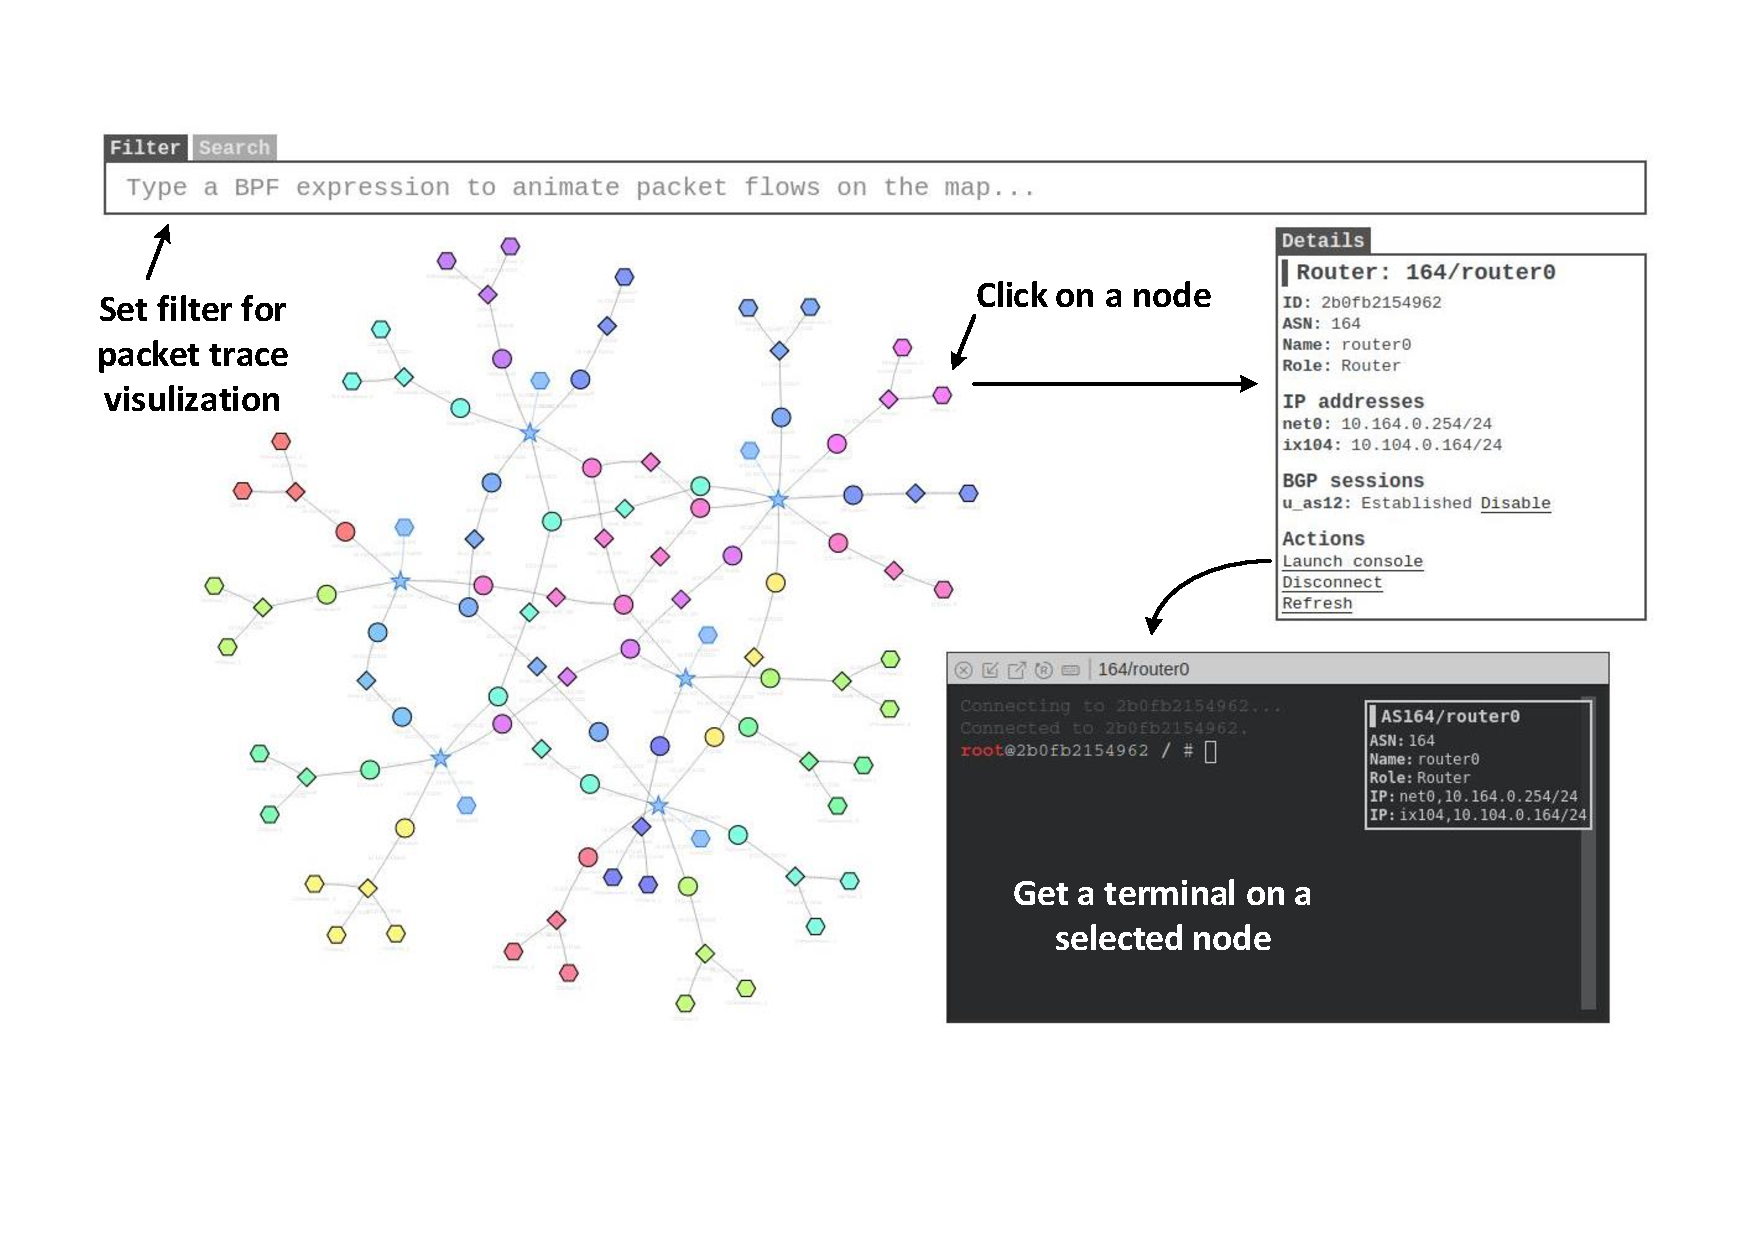
\includegraphics[width=0.95\textwidth]{\bgpFigs/emulator_gui.pdf}
  \end{center}
  \caption{The SEED Internet Emulator}
  \label{bgp:fig:emulator-map}
\end{figure}
 

Each computer (hosts or routers) running inside the emulator is a docker container.
Users can access these computers using docker commands, such as getting a shell
inside a container.
The emulator also comes with a web application, which visualizes all the hosts, routers,
and networks.
After the emulator starts, the map can be accessed from this
URL: \url{http://localhost:8080/map.html}.
See Figure~\ref{bgp:fig:emulator-map}.
Users can interact with this map, such as getting a terminal from any of the container,
disabling BGP sessions (see Figure~\ref{bgp:fig:node-info}). 
Users can also set filters to visualize network traffic.
The syntax of the filter is the same as that in \texttt{tcpdump}; actually,
the filter is directly fed into the \texttt{tcpdump} program running on all nodes.


\begin{figure}[htb]
  \begin{center}
    \includegraphics[width=0.5\textwidth]{\bgpFigs/emulator_node_info.pdf}
  \end{center}
  \caption{Interact with a node}
  \label{bgp:fig:node-info}
\end{figure}
 

% -------------------------------------------
% SUBSECTION
% -------------------------------------------
\subsection{Modifying the BGP Configuration File} 

We need to modify the BGP configuration file in several tasks.
We can do that by directly modifying the configuration file
inside a container. Anther way is to copy the file into the host VM,
do the editing from the host VM, and then copy it back. Let us 
see an example (assuming that we want to modify the BGP configuration
file of AS-180):

\begin{lstlisting}
// Find out the IP of the AS-180's BGP router container
$ dockps | grep 180
6bf0bcda8d06  as180h-host_1-10.180.0.72
437874056b15  as180h-webservice_0-10.180.0.71
(*@\textbf{2967}@*)6d5034ce  as180r-router0-10.180.0.254     (*@\pointleft{This is AS-180's BGP router}@*) 

// Copy the configuration file from the container to the host machine
$ docker cp 2967:/etc/bird/bird.conf ./as180_bird.conf

... edit the file ...

// Copy the file back to the container 
$ docker cp ./as180_bird.conf 2967:/etc/bird/bird.conf 

// Reload the configuration on the container
$ docker exec 2967 birdc configure    (*@\pointleft{Run "birdc configure"}@*) 
BIRD 2.0.7 ready.
Reading configuration from /etc/bird/bird.conf
Reconfigured
\end{lstlisting}
 

% -------------------------------------------
% SUBSECTION
% -------------------------------------------
\subsection{Convention used in the Emulator}

To make it easy to identify the roles of each node in the 
emulator, we have created a set of conventions when assigning
various numbers to nodes. 
These conventions are only for the emulator, and they
do not hold in the real world. 

\begin{itemize}
  \item Autonomous System Number (ASN) assignment:
    \begin{itemize}
      \item ASN \texttt{2 - 9:} for large transit ASes (e.g., national backbone).
      \item ASN \texttt{10 - 19:} for smaller transit ASes.
      \item ASN \texttt{100 - 149:} for Internet Exchanges (IX).
      \item ASN \texttt{150 - 199:} for stub ASes. 
    \end{itemize}

  \item Network prefixes and IP addresses:
    
    \begin{itemize}
      \item For an autonomous system N, its first internal network's prefix
	is \texttt{10.N.0.0/24}, the second internal network
	is \texttt{10.N.1.0/24}, and so on.
   
      \item In each network, the address \texttt{200} to \texttt{255} 
	are for routers. For hosts (non-router), their IP address 
	start from \texttt{71}. For example, in AS-155, 
	\texttt{10.155.0.255} is a BGP router, while \texttt{10.155.0.71}
	is a host. 
    \end{itemize}
     

\end{itemize}



% *******************************************
% SECTION
% *******************************************
\section{Task 1: Stub Autonomous System} 

An autonomous system (AS) is a collection of connected Internet Protocol (IP) routing prefixes
under the control of one or more network operators on behalf of a single administrative entity
or domain. It is a basic unit in BGP. 
A stub AS the type of AS that does not provide transit service to others.
Most of end users are stub ASes, including universities, organization,
and most companies. Another type of AS is called transit AS. They
provide transit services for other ASes, and they 
are Internet service providers.  

In this task, we focus on stub ASes, see how it peers with others. 
For this type of ASes, we will gain a glimpse of how BGP works. 
Students should read Sections \bgpintro - \bgpupdate 
before working on this task. 



 

% -------------------------------------------
% SUBSECTION
% -------------------------------------------
\subsection{Task 1.a: Understanding AS-155's BGP Configuration} 

AS-155 is a stub AS, which has one network (\texttt{10.155.0.0/24})
and one BGP router (\texttt{10.155.0.254}). 
Please  get a terminal on the container of this router, study its 
BGP configuration in \path{/etc/bird/bird.conf}, and then
do the following tasks.

\begin{itemize}
  \item \textbf{Task 1.a.1:} From the BGP configuration file, identify who
    AS-155 peers with. You can ignore the filtering
    part of the configuration for now. Here is one of the
    BGP entries in the configuration file. See Section \bgppeering 
    of the provided BGP tutorial for the explanation of each entry.
    
\begin{lstlisting}
(*@\textbf{protocol bgp}@*) u_as2 {
    ipv4 {
        table t_bgp;
        import filter {
            bgp_large_community.add(PROVIDER_COMM);
            bgp_local_pref = 10;
            accept;
        };
        export where bgp_large_community ~ [LOCAL_COMM, CUSTOMER_COMM];
        next hop self;
    };
    local 10.102.0.155 as 155;
    neighbor 10.102.0.2 as 2;
}
\end{lstlisting}
     

  \item \textbf{Task 1.a.2:} AS-155 peers with several ASes, so if AS-155
    loses the connection with one of them, it can still connect
    to the Internet. Please design an experiment to 
    demonstrate this. You can enable/disable BGP sessions
    either from the graph (see Figure~\ref{bgp:fig:node-info}) or
    using the \texttt{birdc} command (see the following examples). 
    In your experiment, please show how the routing table changes when a particular 
    BGP session is disabled/enabled (you can use the \texttt{"ip route"} to 
    see the content of a routing table). 


\begin{lstlisting}
root@0c97d3ade85a / # birdc show protocols
BIRD 2.0.7 ready.
Name       Proto      Table      State  Since         Info
u_as2      BGP        ---        (*@\textbf{up}@*)     14:51:40.447  Established
u_as4      BGP        ---        up     14:51:39.500  Established

root@0c97d3ade85a / # birdc disable u_as2   (*@\pointleft{Disable peering with AS-2}@*) 
BIRD 2.0.7 ready.
u_as2: disabled

root@0c97d3ade85a / # birdc show protocols
BIRD 2.0.7 ready.
Name       Proto      Table      State  Since         Info
u_as2      BGP        ---        (*@\textbf{down}@*)   16:32:14.883
u_as4      BGP        ---        up     14:51:39.500  Established
\end{lstlisting}

\end{itemize}


% -------------------------------------------
% SUBSECTION
% -------------------------------------------
\subsection{Task 1.b: Observing BGP UPDATE Messages} 

The objective of this task is to understand the BGP UPDATE messages. 
Run \texttt{tcpdump} on AS-150's BGP router,
use it to monitor the BGP traffic. This command will save the 
captured BGP packets into \texttt{/tmp/bgp.pcap}.  

\begin{lstlisting}
# tcpdump -i any -w /tmp/bgp.pcap "tcp port 179"
\end{lstlisting}

Your job is to do something on AS-155's BGP router to trigger
at least one BGP route withdrawal and one BGP route advertisement
messages. These UPDATE messages should be captured by
the \texttt{tcpdump} command on AS-150 and stored inside \texttt{bgp.pcap}.
Copy this file to the host computer using the \texttt{"docker cp"} command (from the host),
and then load it into Wireshark. 
Pick a route advertisement message and a route withdraw message, provide
explanation on these two messages. Screenshots should be provided in the 
lab report.



% -------------------------------------------
% SUBSECTION
% -------------------------------------------
\subsection{Task 1.c: Experimenting with Large Communities} 

When a BGP router sends routes to its peers, they do not send all the routes they
know. What routes are sent depends on many factors, such as the
region of the peers, the business relationship between the peers,
and policies. To help BGP routers make such decisions, additional
information needs to be attached to each route, as the predefined
set of route attributes cannot capture such information.
The BGP Large Communities are created to serve this goal.
The objective of this task is to learn how it is used 
in the emulator to reflect the business relationship
among peers. 

Let us assume that due to some technical issue, 
the connection between AS-4 and AS-156 is broken.  We can
emulate this by disabling the peering between AS-4 and AS-156.
Since AS-4 is the only service provider for AS-156, this essentially
disconnects AS-156 from the Internet. If we ping another host from
one of the hosts in AS-156, we can see the following results (please 
do not run ping from the BGP router; only run it from a host):

\begin{lstlisting}
// On 10.156.0.72
# ping 10.155.0.71
PING 10.155.0.71 (10.155.0.71) 56(84) bytes of data.
64 bytes from 10.155.0.71: icmp_seq=1 ttl=62 time=14.6 ms
64 bytes from 10.155.0.71: icmp_seq=2 ttl=62 time=0.363 ms

# ping 10.161.0.71
PING 10.161.0.71 (10.161.0.71) 56(84) bytes of data.
From 10.156.0.254 icmp_seq=1 Destination Net Unreachable
From 10.156.0.254 icmp_seq=2 Destination Net Unreachable
From 10.156.0.254 icmp_seq=3 Destination Net Unreachable
\end{lstlisting}
 
We can see that \texttt{10.155.0.71} is still reachable, because it
belongs to AS-155, which is still peered with AS-156. However,
\texttt{10.161.0.71} (belonging to AS-161) cannot be reached, because 
nobody will route the packet for AS-156.
The question is, AS-156 still peers with AS-155, 
which is connected to the Internet, so why is AS-156 not able to 
connect to the Internet?  This is because whether an AS forwards 
traffic for another AS depends on their business relationship. 


While AS-156 and AS-4 are trying to solve the problem, AS-156 holds an 
emergency meeting with AS-155, agreeing to pay AS-155, so its 
traffic can temporarily go through AS-155 to reach the Internet. 
This requires some changes on AS-155's BGP router. 
Please make such changes, so AS-155 can temporarily 
provide a transit service to AS-156.
Please read Section \bigcommunity before working on this task. 
After making the changes, please make sure run the following 
command to reload the BIRD configuration.

\begin{lstlisting}
# birdc configure
BIRD 2.0.7 ready.
Reading configuration from /etc/bird/bird.conf
Reconfigured
\end{lstlisting}
 

 
% -------------------------------------------
% SUBSECTION
% -------------------------------------------
\subsection{Task 1.d: Configuring AS-180} 

AS-180 is already included in the emulator. It connects to the
IX-105 Internet exchange (Houston), but it does not peer with anybody, 
so it is not connected to the Internet. 
In this task, students need to complete the configuration of 
AS-180's BGP router and all the related BGP routers, 
so the following goals are achieved:

\begin{itemize}[noitemsep]
  \item Peer AS-180 with AS-171, so they can directly reach each other.
  \item Peer AS-180 with the AS-2 and AS-3 transit autonomous systems, so they can
    reach other destination via these transits.
\end{itemize}

\paragraph{Shell script.}
In this task, we need to modify several BIRD configuration files.
Instead of going to each container to make changes, we can copy
all the BIRD configuration files from the containers to the host VM,
make changes, and then copy them back to the containers.
We have included two shell scripts in the \texttt{task1} folder
to facilitate the process:

\begin{itemize}[noitemsep]
  \item \texttt{import\_bird\_conf.sh}:
    get all the needed BIRD configuration files from the containers.
    If a configuration file already exists in the current folder,
    the file will not be overwritten.

  \item \texttt{export\_bird\_conf.sh}: copy the BIRD configuration
    files to the containers and run \texttt{"birdc configure"}
    to reload the configuration.
\end{itemize}


\paragraph{Debugging.}
If the result is not what you have expected, 
you may need to debug to find out what has gone wrong. In particular, 
you want to know where your packets go. For example, if you run \texttt{ping},
but you do not get a reply, you want to know where the problem is. You can
use the filter option in the map client, and visualize the traffic flow.  
The syntax of the filter is the same as that in \texttt{tcpdump}.
We give a few examples in the following.

\begin{lstlisting}
"icmp"                      (*@\pointleft{show all icmp traffic}@*) 
"icmp and src 10.180.0.71"  (*@\pointleft{show icmp traffic from 10.180.0.71}@*)
"icmp and dst 10.180.0.71"  (*@\pointleft{show icmp traffic  to 10.180.0.71}@*)
\end{lstlisting}
 

\paragraph{Lab report.}
In your lab report, please include the content that you add to the 
BIRD configuration files, and provide proper explanation.
Please also include screenshots (such as traceroute) to demonstrate 
that your task is successful. 



% *******************************************
% SECTION
% *******************************************
\section{Task 2: Transit Autonomous System} 

If two ASes want to connect, they can peer with each other
at an Internet exchange point. The question is how two ASes in two different locations
can reach each other. It is hard for them
to find a common location to peer. To solve this problem,
a special type of AS is needed.

This type of AS have BGP routers in many Internet
Exchange Points, where they peer with many other ASes. Once packets get into
its networks, they will be pulled from one IX to another IX (typically via
some internal routers), and eventually be
handed over to another AS. This type of AS provides the transit
service for other ASes. That is how the hosts in one AS can reach the hosts in
another AS, even though they are not peers with each other.
This special of AS is called \textit{Transit AS}.

In this task, we will first understand how a transit AS works and
then we will configure a transit AS in our Internet emulator. 
Students should read Section \transitas of the tutorial before working on this task.
We pick AS-3 transit autonomous system in this 
task. This AS has four BGP routers, each at a different 
Internet exchange (IX).
We pick the one connected to the Miami Internet exchange (IX-103).

% -------------------------------------------
% SUBSECTION
% -------------------------------------------
\subsection{Task 2.a: Experimenting with IBGP} 

For the task, we first need to find some traffic that 
goes through AS-3. We will ping \texttt{10.164.0.71} from a host in AS-162. Using the 
map client program, we can see that the packets go through
the AS-3 transit AS. If this is not consistent with your observation,
do find some other traffics that go through AS-3. 

We will now disable the IBGP sessions on AS-3's BGP router 
at IX-103 either using the map client or 
from the command line (see the following example).

\begin{lstlisting}
# birdc
bird> show protocols
Name       Proto      Table      State  Since         Info
...
ibgp1      BGP        ---        up     20:19:03.800  Established
ibgp2      BGP        ---        up     20:19:11.921  Established
ibgp3      BGP        ---        (*@\textbf{up}@*)     20:20:50.238  Established

bird> disable ibgp3 
bird> show protocols ibgp3
Name       Proto      Table      State  Since         Info
ibgp3      BGP        ---        (*@\textbf{down}@*)   20:26:44.526
\end{lstlisting}
 
Before disabling IBGP, show the routing table 
on the BGP router (using \texttt{"ip route"}). Compare the 
results before and after disabling IBGP, and explain
your observations. 


% -------------------------------------------
% SUBSECTION
% -------------------------------------------
\subsection{Task 2.b: Experimenting with IGP} 

In this task, we will use the same BGP router. 
We will disable the OSPF routing protocol, and see 
how it affects the routing. There are several ways to disable
OSPF. One way is to do it inside \texttt{birdc}: 

\begin{lstlisting}
# bridc
birdc> show protocols
...
ospf1      OSPF       t_ospf     (*@\textbf{up}@*)     19:49:43.343  Running
...

birdc> disable ospf1
birdc> show protocols ospf1
ospf1      OSPF       t_ospf     (*@\textbf{down}@*)   19:57:37.187
\end{lstlisting}
 
Before and after disabling OSPF, show the routing table 
on the BGP router (using \texttt{"ip route"}). Compare the 
results. Based on the observation, explain why the IGP is essential 
for the transit autonomous systems. 



% -------------------------------------------
% SUBSECTION
% -------------------------------------------
\subsection{Task 2.c: Configuring AS-5} 


\begin{figure}[htb]
  \begin{center}
    \includegraphics[width=0.7\textwidth]{\bgpFigs/as-5.pdf}
  \end{center}
  \caption{AS-5's network diagram}
  \label{bgp:fig:as5}
\end{figure}

The transit autonomous system AS-5 is already included in the emulator. 
It connects to three 
Internet exchanges: IX-101, IX-103, and IX-105,
but it does not peer with any AS. Its topology can be found 
in Figure~\ref{bgp:fig:as5}.
In this task, students need to conduct the following tasks:

\begin{itemize}
  \item The IBGP peering for AS-5 is already established in the 
    emulator. Please use AS-5's BGP router at IX-101 as an example,
    explain the meaning of its IBGP configuration.

  \item AS-5 will provide the transit service for AS-153 (at IX-101), 
    AS-160 (at IX-103), and AS-171 (at IX-105). 
    Please configure their EBGP peering accordingly. Students can 
    learn from the other transit ASes, and see how their peering
    is configured. 


  \item AS-5 and AS-3 are both transit ASes, and they decide to peer at IX-103 (Miami). 
    Since they are roughly the same size, they both benefit from the 
    peering equally, so they decide that
    their relationship should be peer-to-peer, not provider-to-customer.
    They do not pay each other. 
\end{itemize}

In this task, we need to modify several BIRD configuration files.
Just like in Task 1, we have created two shell scripts in the 
\texttt{task2} folder. They can be used to automate the 
downloading/uploading of the BIRD configuration from/to the 
containers.


In your lab report, please include the content you add to the 
BIRD configuration file, and provide proper explanation.
Please also include screenshots (such as traceroute) to demonstrate 
that your task is successful. 



% *******************************************
% SECTION
% *******************************************
\section{Task 3: Path Selection} 

BGP routers typically receive multiple routes to the same network. 
All these routes will be kept, but BGP will run a best route 
selection algorithm to choose one route as the current best route. 
This route will be the one announced to the peers; 
it is also the one given to the kernel routing table, 
so routing is based on this selected route. 
When the best route is retracted, BGP router re-runs the 
best route selection algorithm to find the current best route. 

The top-2 criteria used by BIRD is the following:
(1) prefer route with the highest Local Preference attribute,
(2) prefer route with the shortest AS path. In this task, we will
experiment with these two criteria, and see how they affect 
the path selection. Students should read Section \pathselection 
of the tutorials before working on this task.


\paragraph{Task 3.a.} The \texttt{"birdc show route all > all-routes"} command
can list all the BGP routes (the output is quite long, so it is better to
save the output to a file). The \texttt{"ip route"} command
can list all the entries in the kernel routing table. 

Go to AS-150's BGP router, and show all the BGP routes. Find a network prefix
that has more than one routes. Explain their differences. Compare these 
routes to the entries in the kernel routing table, and identify which route is 
selected as the best route, and explain why this route is selected? 


\paragraph{Task 3.b.}
AS-150 peers with both AS-2 and AS-3, which provide the 
Internet services to AS-150.
However, because the link to AS-2 is slower than
the link to AS-3, AS-150 wants 
to use AS-2 only as the backup upstream link, i.e., 
AS-150's inbound and outbound traffic should 
always use AS-3, unless the link is broken. 
Please modify AS-150's BGP configuration to achieve this goal.



% *******************************************
% SECTION
% *******************************************
\section{Task 4: IP Anycast} 

IP Anycast is a network addressing and routing methodology in which a single
IP address is shared by multiple machines (usually in different locations).
When we send a packet to this IP address, one of the computers will get 
the packet. Exactly which one will get it is hard to tell, because it depends
on the routing. IP anycast is naturally supported by BGP. 
One of the well-known applications of IP anycast is DNS, 
as all 13 root servers A–M exist in multiple locations. 


On the emulator map, type \texttt{190} in the search box, you will find 
out that AS-190 has two networks, but they are disconnected. One network
is connected to IX-100, and the other is connected to IX-105. A closer 
look at these two networks will reveal that these two networks have the 
identical network prefix \texttt{10.190.0.0/24}. The only hosts on
these two networks have the identical IP address \texttt{10.190.0.100}. 

Please find two different hosts in the emulator, so 
when you ping \texttt{10.190.0.100} from these two hosts, 
the destinations are different (even though the destination
IP address is the same). Please set the filter on the map to
\texttt{icmp} to visualize the packet trace, then 
look at the BGP routers on the path, and explain why
the packets reach two different destinations. 
Students should read Section \ipanycast of the tutorial 
before working on this task.



% *******************************************
% SECTION
% *******************************************
\section{Task 5: BGP Prefix Attack} 

BGP Route Hijacking, also called prefix hijacking, is a typical
attack on BGP. In this attack, the attackers' BGP routers 
announce the IP prefix that are not assigned to them, so
the traffic to this IP prefix can get rerouted to the 
attackers, who can intercept or modify the traffic.
Many of the incidents on the Internet are caused by
such an ``attack'', although they are mostly caused 
by the mis-configured BGP routers.
Students should read Section \bgphijacking of the tutorial 
before working on this task.


% -------------------------------------------
% SUBSECTION
% -------------------------------------------
\subsection{Task 5.a. Launching the Prefix Hijacking Attack from AS-161} 

In this task, we will launch the prefix hijacking attack
using a BGP router in AS-161. Our goal is to hijack
the IP prefix owned by AS-154. If the attack is successful,
all the packets going to AS-154 will be rerouted to AS-161, where
they will be dropped. Essentially, we are blackholing AS-154.

In BIRD, the prefixes announced by a BGP router can come from different 
sources: they can come from the \texttt{direct} protocol, 
i.e., they are obtained from the actual network interface attached
to the BGP router. They can also come from the \texttt{static} protocol,
which contains pre-defined routes. The easiest way for a BGP router to 
announce a prefix that it does not own is to use 
the \texttt{static} protocol. The following  
example creates a pre-defined route to \texttt{10.130.0.0/16}. 
See Section \bgpprotocol of the tutorial for detailed explanation of 
the \texttt{static} protocol.
It should be noted that in the filter part of the route,
we need to add the route to the \texttt{LOCAL\_COMM} community; 
otherwise, the BGP router will not export it to the outside.   

\begin{lstlisting}
protocol static {
    ipv4 {
        table t_bgp;
    };
    route 10.130.0.0/16 blackhole { bgp_large_community.add(LOCAL_COMM); };
}
\end{lstlisting}


% -------------------------------------------
% SUBSECTION
% -------------------------------------------
\subsection{Task 5.b. Fighting Back from AS-154} 

AS-154 has a detection system. After the attack was launched,
it immediately detected the attack. It tried to contact
the operators of AS-3, which is the upstream service provider for AS-161,
asking them to block the attack. Unfortunately, it was midnight for AS-3's
operators, so nobody could be reached. The loss of the service
is very significant, so the operators of AS-154 decide to 
fight back: they want to ``steal'' back their own network prefixes, without the help
of AS-3. Please reconfigure the BGP routers of AS-154, so 
you can get the traffic back. 


% -------------------------------------------
% SUBSECTION
% -------------------------------------------
\subsection{Task 5.c. Fixing the Problem at AS-3} 

Eventually, the operators of AS-3 are reached. Without knowing 
whether this is a misconfiguration on the AS-161 side or an intentional
attack, AS-3 decides not to cut the peering with AS-161, so the users 
of AS-161 can still reach the Internet (AS-3 is the only service 
provider to AS-161). However, AS-3 must stop the propagation of the 
fake announcement. This can be done by removing the 
fake routes from its own announcement to its own peers.
More specifically, AS-3 can add some code to its 
filters, so the fake routes can be discarded. 
See Section~\bgphijacking of the BGP tutorial to learn how to write
filters. 


% *******************************************
% SECTION
% ******************************************* 
\section{Submission}

%%%%%%%%%%%%%%%%%%%%%%%%%%%%%%%%%%%%%%%%

You need to submit a detailed lab report, with screenshots,
to describe what you have done and what you have observed.
You also need to provide explanation
to the observations that are interesting or surprising.
Please also list the important code snippets followed by
explanation. Simply attaching code without any explanation will not
receive credits.

%%%%%%%%%%%%%%%%%%%%%%%%%%%%%%%%%%%%%%%%



% *******************************************
% SECTION
% *******************************************
\section*{Acknowledgment} 

This lab was developed with the help of Honghao Zeng, 
a graduate student in the Department of Electrical Engineering 
and Computer Science at Syracuse University. 
The SEED project was funded in part 
by the grants from the US National Science Foundation
and Syracuse University.



\end{document}



